\documentclass[10pt]{article}
\usepackage{tikz}
\usetikzlibrary{shapes.misc}
\usepackage[margin=0cm]{geometry}
\pagestyle{empty}
\tikzstyle{every node}=[cross out, draw, red]

\begin{document}

\vspace*{\fill}
\begin{center}
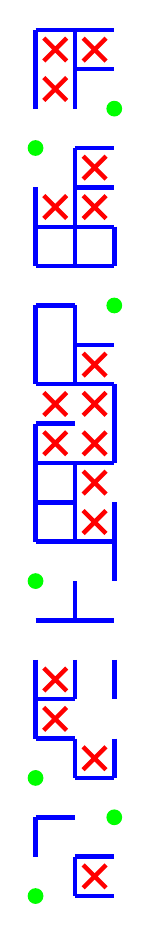
\begin{tikzpicture}[x=0.5cm, y=-0.5cm, ultra thick, blue]
% Walls
    \draw (0,0) -- (2,0);
    \draw (1,1) -- (2,1);
    \draw (1,3) -- (2,3);
    \draw (1,4) -- (2,4);
    \draw (0,5) -- (2,5);
    \draw (0,6) -- (2,6);
    \draw (0,7) -- (1,7);
    \draw (1,8) -- (2,8);
    \draw (0,9) -- (2,9);
    \draw (0,10) -- (1,10);
    \draw (0,11) -- (2,11);
    \draw (0,12) -- (1,12);
    \draw (0,13) -- (2,13);
    \draw (0,15) -- (2,15);
    \draw (0,17) -- (1,17);
    \draw (0,18) -- (1,18);
    \draw (1,19) -- (2,19);
    \draw (0,20) -- (1,20);
    \draw (1,21) -- (2,21);
    \draw (1,22) -- (2,22);
    \draw (0,0) -- (0,2);
    \draw (0,4) -- (0,6);
    \draw (0,7) -- (0,9);
    \draw (0,10) -- (0,13);
    \draw (0,16) -- (0,18);
    \draw (0,20) -- (0,21);
    \draw (1,0) -- (1,2);
    \draw (1,3) -- (1,6);
    \draw (1,7) -- (1,9);
    \draw (1,11) -- (1,13);
    \draw (1,14) -- (1,15);
    \draw (1,16) -- (1,17);
    \draw (1,18) -- (1,19);
    \draw (1,21) -- (1,22);
    \draw (2,5) -- (2,6);
    \draw (2,9) -- (2,11);
    \draw (2,12) -- (2,14);
    \draw (2,16) -- (2,17);
    \draw (2,18) -- (2,19);
% Pillars
    \fill[green] (2,2) circle(0.2);
    \fill[green] (0,3) circle(0.2);
    \fill[green] (2,7) circle(0.2);
    \fill[green] (0,14) circle(0.2);
    \fill[green] (0,19) circle(0.2);
    \fill[green] (2,20) circle(0.2);
    \fill[green] (0,22) circle(0.2);
% Inner points in accessible cul-de-sacs
    \node at (0.5,0.5) {};
    \node at (1.5,0.5) {};
    \node at (0.5,1.5) {};
    \node at (1.5,3.5) {};
    \node at (0.5,4.5) {};
    \node at (1.5,4.5) {};
    \node at (1.5,8.5) {};
    \node at (0.5,9.5) {};
    \node at (1.5,9.5) {};
    \node at (0.5,10.5) {};
    \node at (1.5,10.5) {};
    \node at (1.5,11.5) {};
    \node at (1.5,12.5) {};
    \node at (0.5,16.5) {};
    \node at (0.5,17.5) {};
    \node at (1.5,18.5) {};
    \node at (1.5,21.5) {};
% Entry-exit paths without intersections
\end{tikzpicture}
\end{center}
\vspace*{\fill}

\end{document}
